\documentclass[11pt]{article}
\usepackage[english]{babel}
\usepackage{url}
\usepackage{graphicx,DCCN2019_en}
\usepackage{placeins}

\pagestyle{fancy}
\fancyhead{} 
\fancyfoot{}

\usepackage[utf8]{inputenc}
\linespread{1.0}

\usepackage{amsmath}

\makeatletter
\fancyhead[RO]{\small DCCN 2019 \\ {23-27 September 2019}}
\fancyhead[LO]{\small Ketipov, Kostadinov, Petrov, Zankinski, Balabanov \\ Human-Computer MDC for TS Forecasting}
% Rumen Ketipov
% Georgi Kostadinov
% Plamen Petrov
% Iliyan Zankinski
% Todor Balabanov

\c@page=1 
       
\makeatother

\title{Human-Computer Mobile Distributed Computing for Time Series Forecasting}

\author[1]{\small R.R. Ketipov}
\author[1]{\small G.B. Kostadinov}
\author[1]{\small P.D. Petrov}
\author[1]{\small \\I.A. Zankinski}
\author[0000-0003-3139-069X]{\small T.D. Balabanov}

\affil[1]{\footnotesize Institute of Information and Communication Technologies (IICT) \break Bulgarian Academy of Sciences (BAS) \break acad. Georgi Bonchev Str., block 2, 1113 Sofia, Bulgaria}

\email{rketipov@iit.bas.bg, g.kostadinov@iit.bas.bg, p.petrov@iit.bas.bg, iliyan@hsi.iccs.bas.bg, todorb@iinf.bas.bg}

\begin{document}

\udc{004.93}

{\let\newpage\relax\maketitle}

\vskip -1.5em

\footnotetext{This work was supported with private funding by Velbazhd Software LLC.}

\begin{abstract}
Distributed computing became very popular in the last two decades. In many cases distributed computing projects are based on a donated calculation power. One of the most famous donated distributed computing project is SETI@home, which is related to deep space signals processing in attempt to find an alien life. The usage of donated distributed computing had its influence in the time series forecasting in the face of MoneyBee\cite{bohn01} project. MoneyBee project was a desktop screensaver application, which was calculating financial time series forecasting by training of artificial neural networks with evolutionary algorithms. With the expansion of the mobile devices in the last decade it become relevant some donated distributed computing solutions to be developed as mobile applications. Such a solution was developed at IICT-BAS\cite{tomov01}, which is based on Android Live Wallpaper technology. This research proposes an extension of the work done at IICT-BAS in the direction of human-computer based distributed computing by providing software capabilities of the users to vote for future financial changes. 

\keywords{distributed computing, time series forecasting, artificial neural networks, evolutionary algorithms}
\end{abstract}

\section{Introduction} \label{Introduction}

Financial time series forecasting is an attractive and intensively researched area \cite{nava01}. One of the most interesting research directions in this field is related to the usage of artificial neural networks combined with evolutionary algorithms \cite{zhang01}. In some studies evolutionary algorithms are used for artificial neural network topology optimization \cite{kapanova01}, but in other studies evolutionary algorithms are used for artificial neural network weights optimization \cite{aljarah01}. When evolutionary algorithms are used for weights optimization it is very common the training to be combined with back-propagation algorithm. Even when such a hybrid training algorithm is used it is in the class of supervised training. Training examples are fed to the artificial neural network and its weights are modified according the selected training algorithm. Evolutionary algorithms have a common advantage compared to the exact numerical methods and that is the possibility for parallel calculations \cite{altinoz01}. When the parallel calculations are done on separate mobile devices it is the case of mobile distributed computing. It is very common the financial forecasting to be done by the usage of the past values in the time series, but it can be also combined with human evaluation of the future values. In this research a human-computer based mobile distributed computing solution is proposed. The users are using an Android application which trains artificial neural network with evolutionary algorithms and back-propagation, but users are capable to vote for increase or decrease of the future values. The most successful forecast votes of the users are used in artificial neural network training process.

\section{Model Proposition} \label{Model Proposition}

MoneyBee screensaver (Fig. \ref{fig01}) was organized as a desktop application, which runs in background when the computer is in idle mode. Artificial neural networks were trained with the usage of evolutionary algorithms. The main advantage of this approach is that it is using donated computation power of many participants. In the same time the biggest disadvantage is that the screensaver is used relatively rare, only when the user is not using the computer. The other disadvantage is that personal computers are not used 24/7.

\begin{figure}
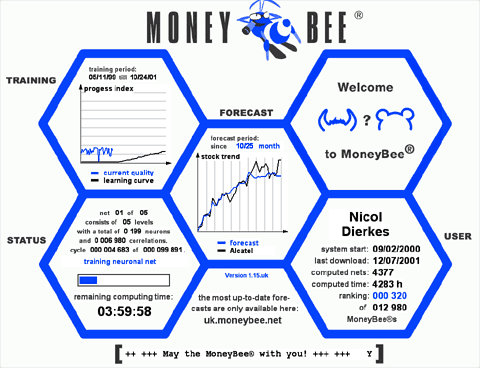
\includegraphics[width=0.5\textwidth]{fig01.png}
\centering
\caption{MoneyBee screensaver} \label{fig01}
\end{figure}
\FloatBarrier

These disadvantages are addressed in the VitoshaTrade project (Fig. \ref{fig02}), developed in IICT-BAS. The implementation is done under an Android operating system as active wallpaper. Inside the forecasting module a multilayer perceptron is used. The training algorithm is a combination between back-propagation and differential evolution. All calculations are done as active Android application, which works 24/7 in a background mode. When better artificial neural network weights are found a communication with a remote server is established. Active wallpapers are used to visualize information on a full screen behind all other visual components. 

\begin{figure}
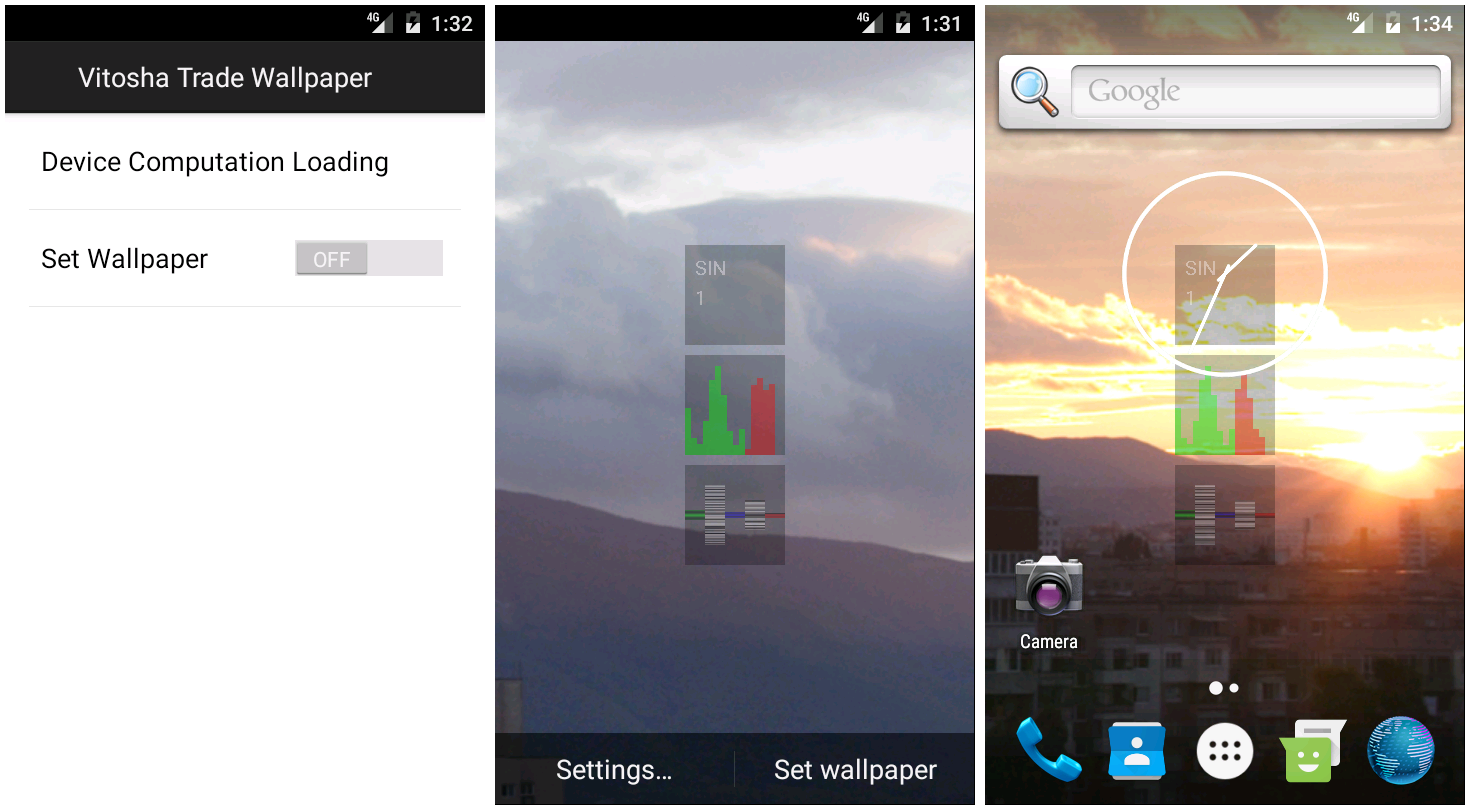
\includegraphics[width=1.0\textwidth]{fig02.png}
\centering
\caption{VitoshaTrade active wallpaper} \label{fig02}
\end{figure}
\FloatBarrier

In both projects only a pure mathematical information is used for prediction calculations. This limitation was overcome in ElectricSheep\cite{draves01} project. In this project it is used a rating system whereat the users vote for different fractal generated animations. Voting is done in two directions - thumb up and thumb down. Each vote increases or decreases individual rating, which is directly related to its survival chances. The rating is not constant and it goes down with the time passing. 

This study proposes a combination of the projects described above. The VitoshaTrade project is extended in the direction of voting system addition. The Android operating system offers software modules called widgets. Widgets have graphical user interface and they occupy small part of the visible working area. Most commonly widgets are used for representation of small pieces of information, such astronomical time, weather forecast, calendar and many others. Widgets are much more interactive than the active wallpaper. The user is capable to input small pieces of information as voting for example. The other better advantage of the widgets is that users have much better control over visualization and placement of the widgets. In this study a composite widget is proposed, which shows the thicker of the currency pair (EUR/USD in the example provided), the value of the rate between the two currencies, and arrows for vote up or vote down. 

Voting of the users is collected on PHP/MySQL based web server\cite{tomov01}, a part of the server side implementation of the VitoshaTrade project. On the server side additional analysis is done. Votes which were more accurate are better taken for next generations in the global distributed differential evolution population. 

\section{Experiments} \label{Experiments}

Experiments are done with FOREX financial time series of EUR/USD currency pair (Fig. \ref{fig03}). Time series is disassembled in training examples (7 values for lag and 3 values for lead). A back-propagation combined with differential evolution training of multilayer perceptron is done. The training process is continuous, which means that the forecasting is done parallel with the training. The voting of the user directly influences the fitness value of the individuals in the distributed differential evolution population. Some users are better in their vision and are more successful during the voting process, therefore the tracking of the users is of great importance. More reliable votes are taken with higher coefficient for the further predictions. According to some regulations, like GDPR in EU \cite{hristov01}, a special care should be taken for the personal information collected on the servers side. 

\begin{figure}
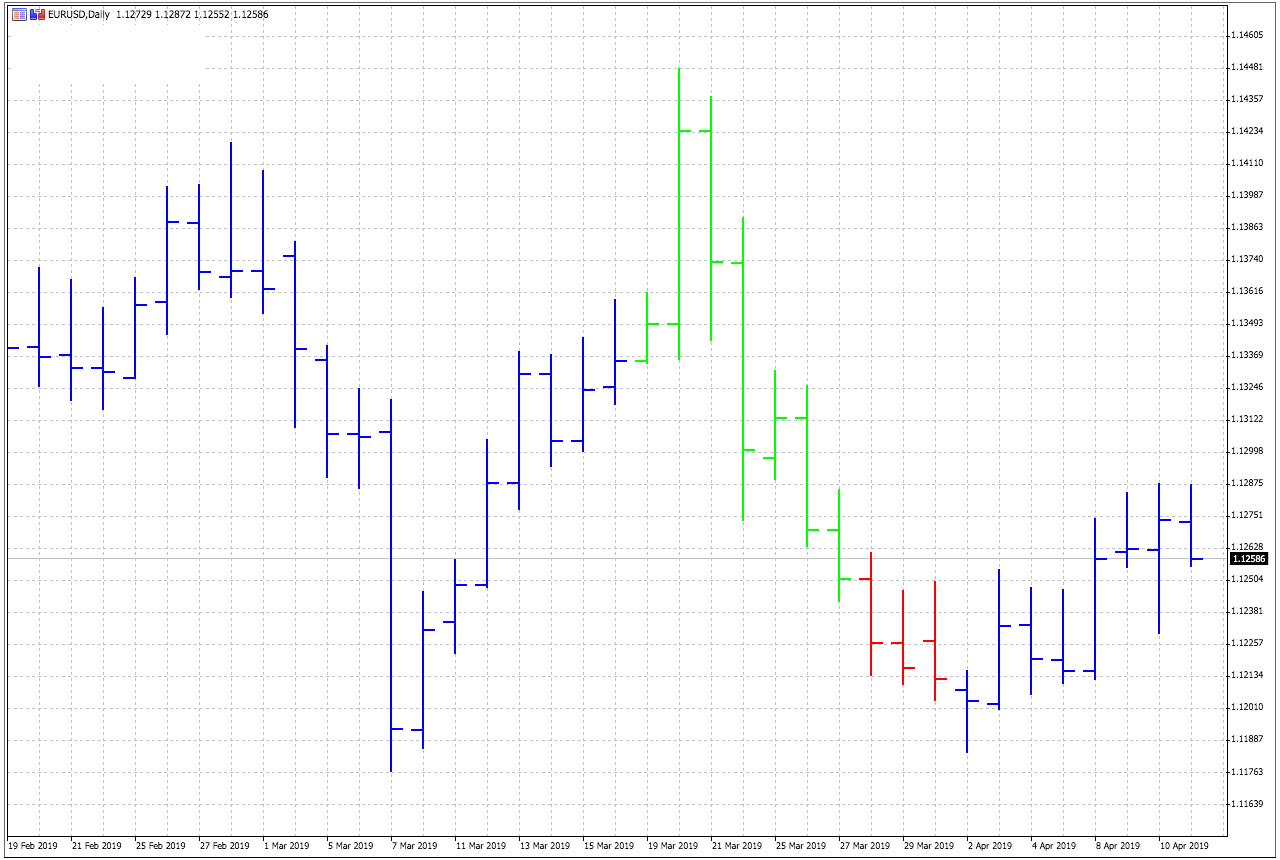
\includegraphics[width=0.8\textwidth]{fig03.png}
\centering
\caption{Forex EUR/USD time series.} \label{fig03}
\end{figure}
\FloatBarrier

\section{Conclusion} \label{Conclusion}

Pure technical analysis in time series field has its limits. Values measured in time are just one projection of the process which goes under it. Any computer based calculation nowadays is not capable to act as human intuition. The mechanisms behind human intuition are not investigated enough and are still very difficult to recreate in the modern computers. Because of these reasons the proposed financial time series forecasting solution advances the pure technical analysis with minimal influence of human impact. The proposed simple voting system consolidated the power of machine learning algorithms and the human sixth sense feeling in an efficient and cost effective financial forecasting infrastructure.

As a future research it will be interesting different communication capabilities to be investigated as described in \cite{alexandrov01}. Also it will be interesting generalized artificial neural networks \cite{tashev01} to be used instead of multilayer perceptron.

\vskip 1.5em

\begin{thebibliography}{99}

\bibitem{nava01} Nava, N., Di Matteo, T., Aste, T., \textbf{\textit{Financial Time Series Forecasting Using Empirical Mode Decomposition and Support Vector Regression}}, RISKS, \textbf{6}(1), article 7, 2018.

\bibitem{zhang01} Zhang, R., Tao, J., \textbf{\textit{A Nonlinear Fuzzy Neural Network Modeling Approach Using an Improved Genetic Algorithm}}, IEEE Transactions on Industrial Electronics, \textbf{65}(7), p. 5882--5892, 2018.

\bibitem{kapanova01} Kapanova, K., Dimov, I., Sellier, J.M., \textbf{\textit{A genetic approach to automatic neural network architecture optimization}}, Neural Computing and Applications, Springer London, \textbf{29}(5), p. 1481--1492, 2016.

\bibitem{aljarah01} Aljarah, I., Faris, H., Mirjalili, S., \textbf{\textit{Optimizing connection weights in neural networks using the whale optimization algorithm}}, Soft Computing, Springer Berlin Heidelberg, \textbf{22}(1), p. 1–15, 2016.

\bibitem{altinoz01} Altinoz, O.T., Deb, K., \textbf{\textit{Late parallelization and feedback approaches for distributed computation of evolutionary multi-objective optimization algorithms}}, Neural Computing and Applications, Springer London, \textbf{30}(3), p. 723--733, 2016.

\bibitem{bohn01} Bohn, A., Guting, T., Mansmann, T., \textbf{\textit{MoneyBee: A new product to predict stock market developments using artificial intelligence and increased calculation capacitiy}} (in German), et al. Wirtschaftsinf, \textbf{45}(3), p. 325--333, 2003.

\bibitem{tomov01} Tomov, P., Zankinski, I., Barova, M., \textbf{\textit{Mobile Alternative of the MoneyBee Project for Financial Forecasting}}, Proceedings of the Annual University Scientific Conference of the National Military University Vasil Levski, Veliko Tarnovo, p. 1085--1089, 2018.

\bibitem{hristov01} Hristov, P., Dimitrov, W., \textbf{\textit{The blockchain as a backbone of GDPR compliant frameworks}}, Proceedings of 8th International Multidisciplinary Symposium - Challenges and Opportunities For Sustainable Development Through Quality and Innovation in Engineering and Research Management, \textbf{20}(1), p. 305--310, 2018.

\bibitem{draves01} Draves, S., \textbf{\textit{The Electric Sheep Screen-Saver: A Case Study in Aesthetic Evolution}}, Proceedings of Applications of Evolutionary Computing: EvoWorkkshops: EvoBIO, EvoCOMNET, EvoHOT, EvoIASP, EvoMUSART, and EvoSTOC Lausanne, LNCS 3449, p. 458--467, 2005.

\bibitem{alexandrov01} Alexandrov, A., \textbf{\textit{Comparative analysis of IEEE 802.15.4 based communication protocols used in wireless intelligent sensor systems}}, Proceedings of the International conference RAM, p. 51--54, 2014.

\bibitem{tashev01} Tashev, T., Hristov, H., \textbf{\textit{Modeling of synthesis of information processes with generalized nets}}, Cybernetics and Information Technologies, \textbf{3}(2), p. 92--104, 2003.

\end{thebibliography}

\end{document}
